\documentclass[11pt]{article}
\usepackage[UTF8]{ctex}
\usepackage[a4paper]{geometry}
\geometry{left=2.0cm,right=2.0cm,top=2.5cm,bottom=2.5cm}

\usepackage{comment}
\usepackage{booktabs}
\usepackage{graphicx}
\usepackage{diagbox}
\usepackage{amsmath,amsfonts,graphicx,amssymb,bm,amsthm}
\usepackage{algorithm,algorithmicx}
\usepackage[noend]{algpseudocode}
\usepackage{fancyhdr}
\usepackage{tikz}
\usepackage{graphicx}
\usepackage{verbatim}
\usetikzlibrary{arrows,automata}
\usepackage{hyperref}

\setlength{\headheight}{14pt}
\setlength{\parindent}{0 in}

\newtheorem{theorem}{Theorem}
\newtheorem{lemma}[theorem]{Lemma}
\newtheorem{proposition}[theorem]{Proposition}
\newtheorem{claim}[theorem]{Claim}
\newtheorem{corollary}[theorem]{Corollary}
\newtheorem{definition}[theorem]{Definition}


\newcommand\E{\mathbb{E}}
\newcommand{\hwid}{2}			% 第几次作业
\newcommand{\name}{周雨扬} 		% 你的名字
\newcommand{\id}{2000013061} 	% 你的学号


\usetikzlibrary{positioning}

\begin{document}

    \pagestyle{fancy}
    \lhead{Peking University}
    \chead{}
    \rhead{Operating Systems}

    \begin{center}
        {\LARGE \bf Homework \#\hwid}\\
        {\Large \name}\\
        {\Large \id}\\
    \end{center}

	\section{Challanges}
		\par 本次作业完成了所有的代码补全任务,做了如下的 Challange:
		\begin{itemize}
			\item Display in a useful and easy-to-read format all of the physical page mappings (or lack thereof) that apply to a particular range of virtual/linear addresses in the currently active address space. For example, you might enter \texttt{showmappings 0x3000 0x5000} to display the physical page mappings and corresponding permission bits that apply to the pages at virtual addresses \texttt{0x3000}, \texttt{0x4000}, and \texttt{0x5000}.
			\item Explicitly set, clear, or change the permissions of any mapping in the current address space.
		\end{itemize}
		
	\section{Exercise 1}
	
	\subsection*{boot\_alloc()}
		\par 该部分代码需要初始的时候设置用于声明一级页表,以及管理二级页表的链表的内存(事实上没有声明二级页表),等待两者初始化完毕后再利用这个没有建立完的二级页表进行寻址。由于初始没有二级页表,这部分即用于声明二级页表,以及页管理链表的内存。
		
		\par 虽然代码中,声明的内存只有大约 \texttt{4 MB},远不会超出内存限制;但是安全起见还是加上了防止内存溢出的设置。代码可以见 \texttt{kern/pmap.c, Line 106 $\sim$ 117}。
		
	\subsection*{mem\_init()}
		\par 此时我们只需要声明用于存储页链表 \texttt{pages} 的内存即可。因此可以通过直接调用 \texttt{boot\_alloc} 解决。代码可以见 \texttt{kern/pmap.c, Line 163 $\sim$ 165}。
		
	\subsection*{page\_init()}
		\par 这里我们需要初始化链表。观察链表元素我们发现 \texttt{pp\_ref} 是表示页被多少玩意引用的,如果是 0 则代表是一个空页;同时 \texttt{pp\_link} 记录了空页链表的下一个页的链接,如果其不是空页则指针为空。
		
		\par 根据信息知道此时候只有三部分已经使用的页:第一部分是一级页表,共1页;第二部分是IO缓冲区,界限已经给出;第三部分是我们声明链表的内存(有可能还包括其他的),界限可以通过调用 \texttt{boot\_alloc()} 获得。
		
		\par 据此我们可以根据界限分类声明即可,代码可以见 \texttt{kern/pmap.c, Line 269 $\sim$ 292}。
		
	\subsection*{page\_alloc()}
		\par 这里我们需要支持页分配;此时我们只需要从 \texttt{page\_init()} 预处理出来的 \texttt{page\_free\_list} 中寻找即可,注意链表维护的细节即可。代码可以见 \texttt{kern/pmap.c, Line 312 $\sim$ 320}。
	
	\subsection*{page\_free()}
		\par 这里我们需要支持页收回。我们需要通过检查 \texttt{pp\_ref} 是否为 0 来判断是否仍有页引用;需要通过检查 \texttt{pp\_link} 判断该页是否已经在空列表中。如果满足条件,则直接将其加入列表即可。代码可以见 \texttt{kern/pmap.c, Line 333 $\sim$ 338}。
		
	\section{Exercise 4}
	
	\subsection*{pgdir\_walk()}
		\par 这部分需要我们检索二级页表,如果其不存在且需要创建则声明对应的页。
		\par 首先我们检索一级页表,如果一级页表中 \texttt{PTE\_P} 位为真,则表示其对应的二级页表存在,直接根据访存地址即可确定存储页信息的位置;
		如果一级页表不存在,且我们需要创建,则我们首先需要声明一页用于存储二级页表,修改一级页表的信息,修改页引用数,最后返回存储页信息的地址。
		
		\par 注意返回地址时候的,对地址进行加法操作的时候指针类型。代码可以见 \texttt{kern/pmap.c, Line 378 $\sim$ 394}。
		
	\subsection*{boot\_map\_region()}
		\par 这部分需要将一段连续虚拟地址映射到连续物理地址上,同时设置权限位信息。
		\par 首先利用 \texttt{pgdir\_walk()}, 我们找到所虚拟地址对应的所有的页,如果不存在上述的页还需要将其创建。之后根据返回的地址,我们只需要修改其映射的物理地址,以及其对应的权限位即可。
		\par 代码可以见 \texttt{kern/pmap.c, Line 412 $\sim$ 417}。
		
	\subsection*{page\_lookup()}
		\par 这部分需要将在二级页表中查询虚拟地址对应的页信息,以及对应的二级页表的地址。
		
		\par 利用 \texttt{pgdir\_walk()} 查询的结果,如果存在于页表中,且  \texttt{PTE\_P} 位为真,则说明其存在,返回对应信息即可;否则返回不存在。代码可以见 \texttt{kern/pmap.c, Line 476 $\sim$ 486}。
		
	
	\subsection*{page\_remove()}
		\par 这部分需要删除虚拟地对应的页。
		\par 注意在删除的时候,虽然可能页引用数量仍不为 0,其仍需要在页表中删除。代码可以见 \texttt{kern/pmap.c, Line 508 $\sim$ 515}。
	
	\subsection*{page\_insert()}
		\par 这部分需要加入虚拟地对应的页。
		\par 此时我们不仅需要查询对应的页,还需要在该页已经存在的时候删除原有的页映射信息;删除后既可以通过修改对应映射信息来插入。
		\par 注意,我们不仅需要加入二级页表的权限信息,还需要将对应的修改一级页表的权限。代码可以见 \texttt{kern/pmap.c, Line 448 $\sim$ 457}。
	
	
	\section{Exercise 5}
	
	\subsection*{mem\_init()}
		\par 此时我们可以直接使用 \texttt{boot\_map\_region} 进行虚拟内存到物理内存的映射。这里我们注意到我们没有必要进行栈缓冲区的映射,因为其不映射的话在寻址的时候就会报错,确实能够完成缓冲的问题。
	
		\par 代码可以见 \texttt{kern/pmap.c, Line 189,201,211}。
		
	\section{Question}
	
	\subsection*{Question 1}
		\par \texttt{uintptr\_t},因为 \texttt{T*} 的类型是 \texttt{uintptr\_t}
		
	\subsection*{Question 2}
	\par 
	\texttt{Block 961$\sim$1024, Address 0xf0000000$\sim$0xfffffff} 最顶上的 $64$ 个一级页表,将虚拟内存映射到了 \texttt{256MB} 的物理内存中。
	\par 
	\texttt{Block 960, Address 0xefc00000 $\sim$ 0xefffffff}, 映射了内核栈,内核信息等所处的内存。
		
	\subsection*{Question 3}
	\par 第 $1$ 段一级页表映射了包括一级页表,二级页表,页链表等的信息的,
	
	\par 由于二级页表中每一个存储信息的结构 \texttt{pte\_t} 中有 $12$ 位的专门用于存储权限的内存空间,这些比特表示用户/系统是否有权限来对这页的信息进行相关操作。
	
	\par 在 \texttt{mem\_init} 中我们一开始已经设定了存储内核信息,内核栈的部分的权限,我们将其设置为不可阅读。因此在用户权限的进程尝试访问的时候,系统会终止访问并返回错误。 
	
	
	\subsection*{Question 4}
	
	\par 该内核共有 1 个一级页表,1024 个二级页表,至多 $2^20$ 个大小为 $4KB$ 的页,因此能够管理的内存至多有 $4GB$。
	
	\subsection*{Question 5}
	
	\par 初始其会声明至多 $8MB$ 用于存储页链表信息,$4MB$ 用于二级页表, $4MB$ 用于一级页表。 
	
	\subsection*{Question 6}
	
	\par 代码片段位于 \texttt{kern/entry.S, Line 67 $\sim$ 69}
	\par 没有设置的时候内存映射中虚拟内存 $[0,4MB]$ 被映射到了物理内存 $[0,4MB]$,因此以一个较低的 \texttt{EIP} 运行不会产生问题,但是在设置后虚拟内存 $[0,4MB]$ 便不再允许随意调用了。
	
	\section{Challange Implementation}
	
	\subsection*{challange 1}
	
	\par 第一个challange我们需要逐页的输出某一段连续虚拟地址对应的物理地址位置信息,访问权限,以及在不存在上述映射时候返回错误信息。最终实现效果如下:
	
	
\begin{figure}[htbp]
\centering
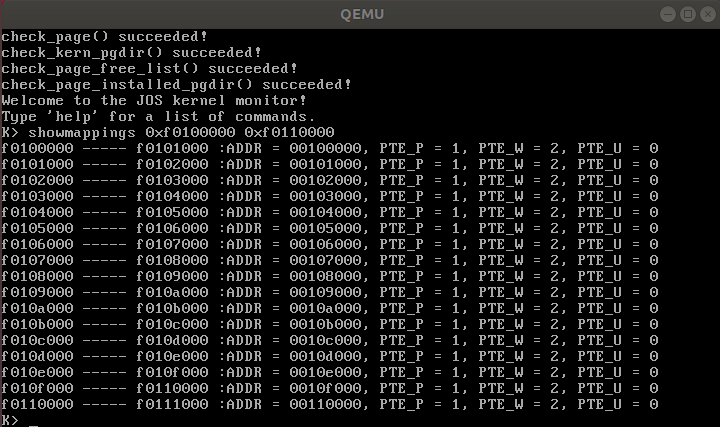
\includegraphics[width=0.7\linewidth]{lab2-cha1.png}
\end{figure}

\par 代码可以见 \texttt{kern/moniter.c, Line 95 $\sim$ 129}。
	\subsection*{challange 2}
	
	\par 第二个challange我们需要修改某一个页表的权限位,最终实现效果如下:
		
		\begin{figure}[htbp]
			\centering
			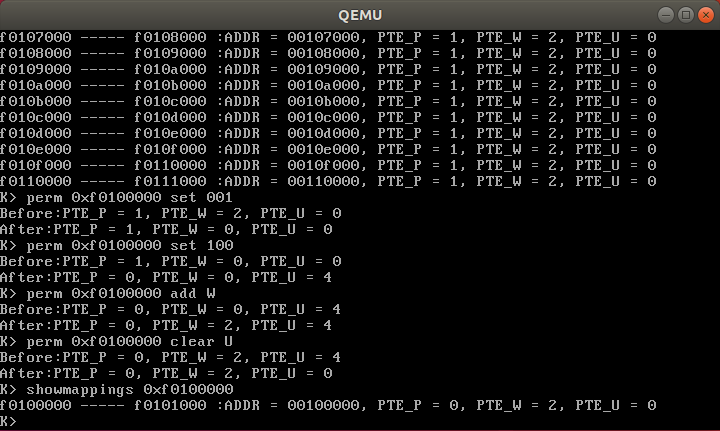
\includegraphics[width=0.7\linewidth]{lab2-cha2.png}
		\end{figure}
		
		\par 代码可以见 \texttt{kern/moniter.c, Line 133 $\sim$ 175}。
\end{document}